% !TeX root = _main.tex
% DE XUAT CUA TV1 CHO MUC TO-BE (Batch 3) -- TV3 duyet roi moi ghep.
% File nay CHUA duoc \input o dau, nen khong anh huong PDF hien tai.
% Cach ghep (TV3): trong role_3.tex, xoa khoi tu dong "\subsection{Quy trình TO-BE}"
% den truoc dong "\FloatBarrier" ngay tren "\section{Đánh giá, độ nhạy và giới hạn}",
% roi thay bang mot dong: % !TeX root = _main.tex
% DE XUAT CUA TV1 CHO MUC TO-BE (Batch 3) -- TV3 duyet roi moi ghep.
% File nay CHUA duoc \input o dau, nen khong anh huong PDF hien tai.
% Cach ghep (TV3): trong role_3.tex, xoa khoi tu dong "\subsection{Quy trình TO-BE}"
% den truoc dong "\FloatBarrier" ngay tren "\section{Đánh giá, độ nhạy và giới hạn}",
% roi thay bang mot dong: % !TeX root = _main.tex
% DE XUAT CUA TV1 CHO MUC TO-BE (Batch 3) -- TV3 duyet roi moi ghep.
% File nay CHUA duoc \input o dau, nen khong anh huong PDF hien tai.
% Cach ghep (TV3): trong role_3.tex, xoa khoi tu dong "\subsection{Quy trình TO-BE}"
% den truoc dong "\FloatBarrier" ngay tren "\section{Đánh giá, độ nhạy và giới hạn}",
% roi thay bang mot dong: % !TeX root = _main.tex
% DE XUAT CUA TV1 CHO MUC TO-BE (Batch 3) -- TV3 duyet roi moi ghep.
% File nay CHUA duoc \input o dau, nen khong anh huong PDF hien tai.
% Cach ghep (TV3): trong role_3.tex, xoa khoi tu dong "\subsection{Quy trình TO-BE}"
% den truoc dong "\FloatBarrier" ngay tren "\section{Đánh giá, độ nhạy và giới hạn}",
% roi thay bang mot dong: \input{role_1_tobe}
% Nhan cu \label{r3:bpmn} khong duoc tham chieu o dau khac nen xoa duoc.
% So do: figures/r1_bpmn_tobe.bpmn (sua tren demo.bpmn.io), ban PDF: figures/r1_bpmn_tobe.pdf.

\subsection{Quy trình TO-BE và quy tắc vận hành}
\label{r1:tobe}
TO-BE gồm hai lớp thay đổi. Lớp thứ nhất áp dụng cho mọi khách: số kênh $c_t$ đổi theo
giờ theo Bảng~\ref{r3:staffing} (A1, và A2 khi có số hóa), do cửa hàng trưởng công bố
trước. Lớp thứ hai là thay đổi quy trình cho khách dùng ứng dụng (A2): đơn được chuẩn bị
trước khi vào trụ, tại trụ nhân viên chỉ quét mã, kiểm tra vòi, hệ thống trừ tiền rồi
mới bơm đúng số tiền; HĐĐT gửi về ứng dụng. Khách không dùng ứng dụng, hoặc trừ tiền
không thành công, đi theo luồng AS-IS ở Hình~\ref{r1:bpmn}, nên kênh tiền mặt vẫn được giữ.
Hình~\ref{r1:tobe-bpmn} và Bảng~\ref{r1:tobe-changes} cho biết bước nào đổi, ai chịu
trách nhiệm và thay đổi tác động lên biến nào của mô hình.

\begin{figure}[p]\centering
\rotatebox{90}{\begin{minipage}{\textheight}\centering
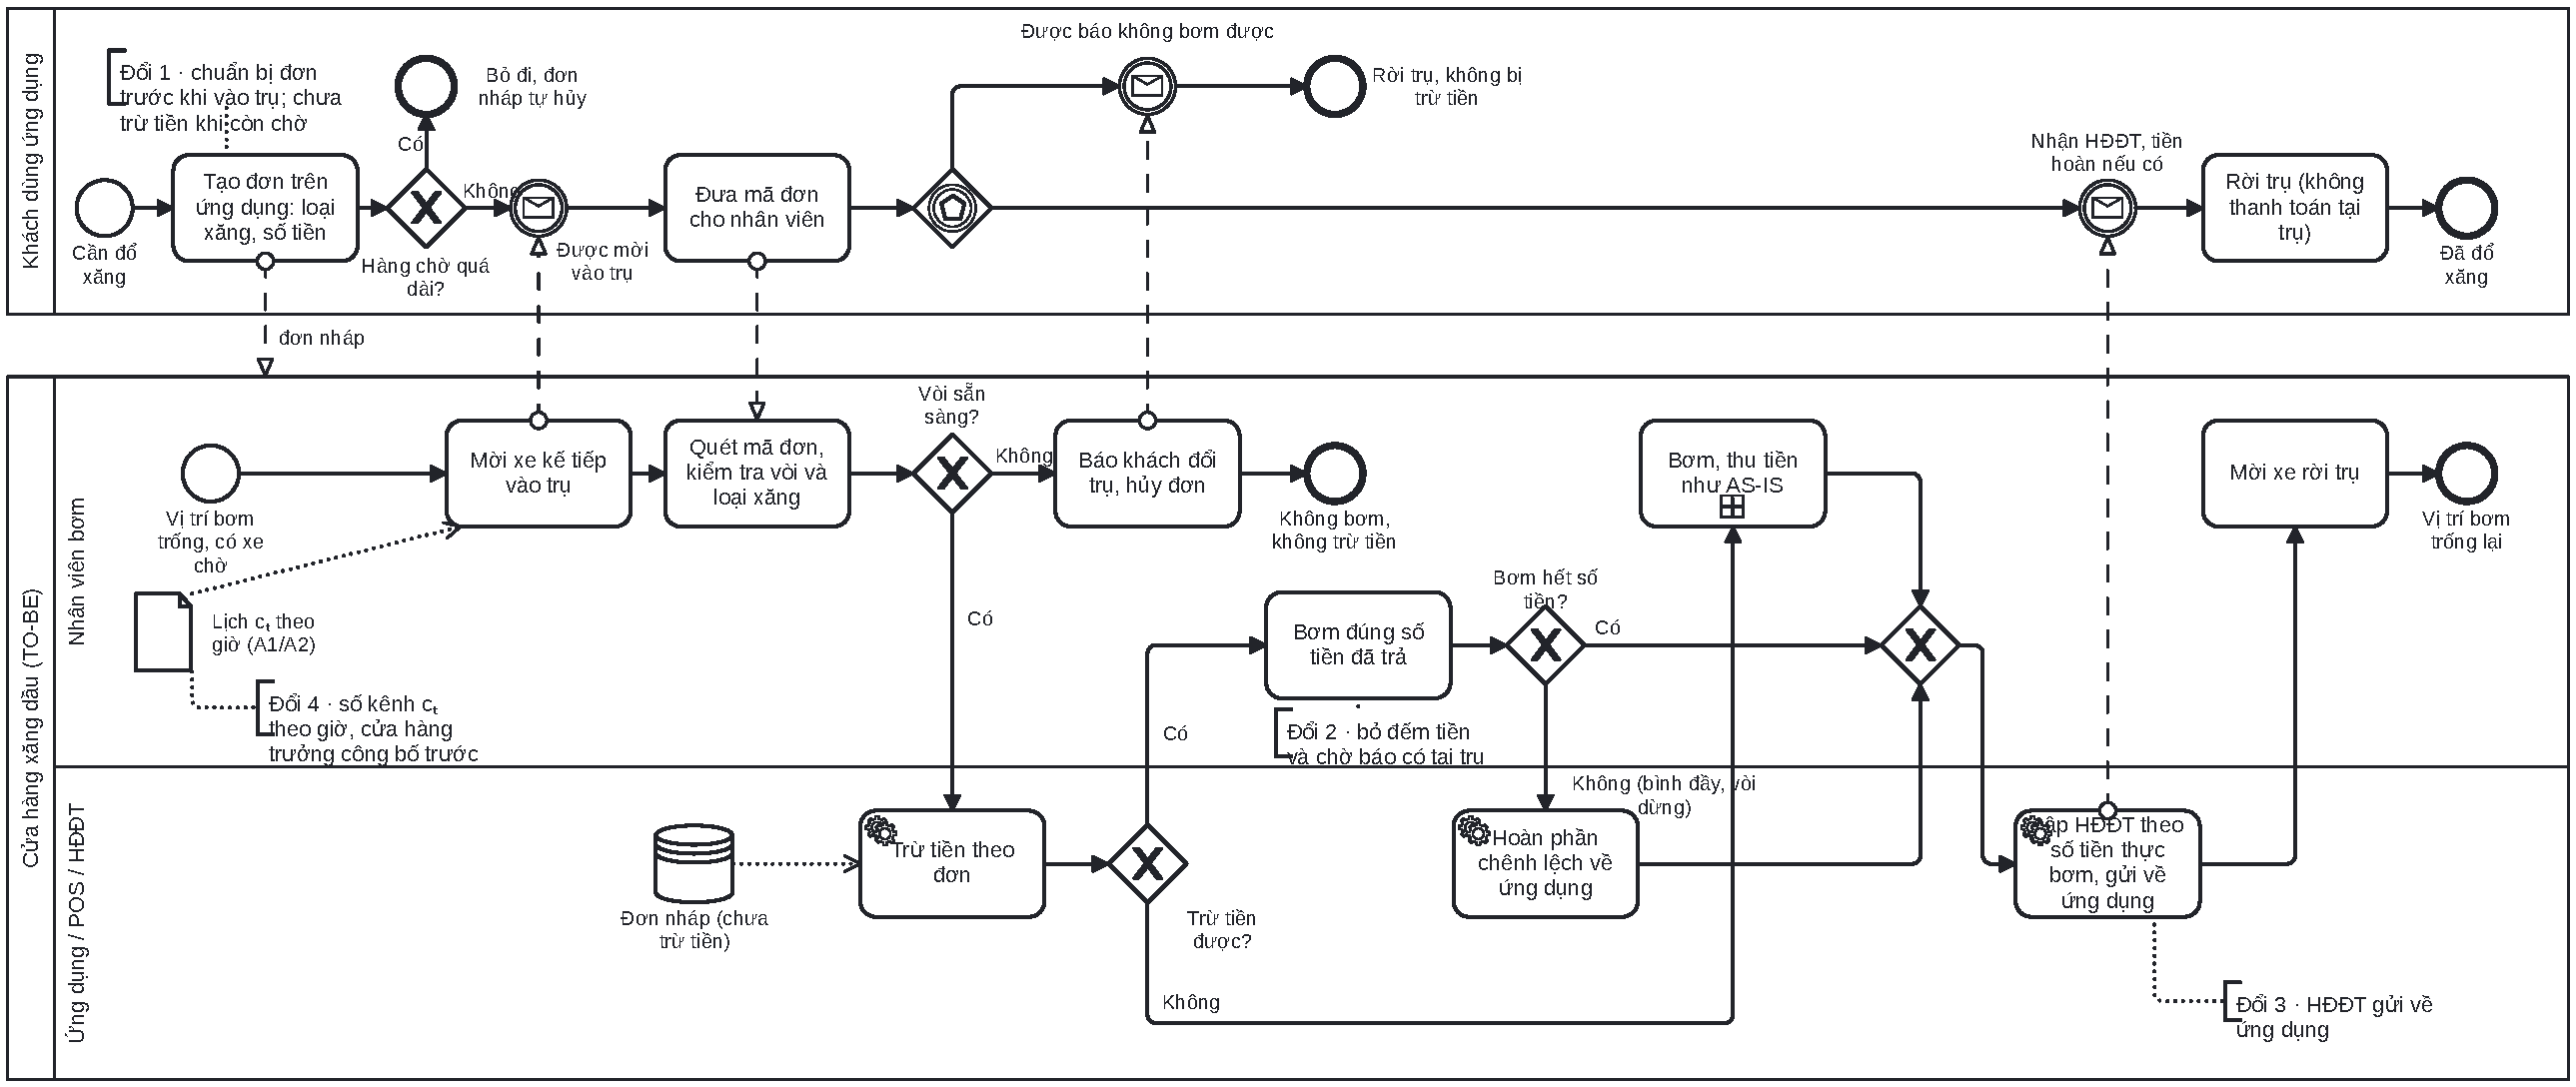
\includegraphics[width=0.86\linewidth]{figures/r1_bpmn_tobe.pdf}
\captionof{figure}{BPMN TO-BE cho khách dùng ứng dụng trả trước; ``Đổi 1--4'' là thay đổi so với AS-IS,
khối có dấu $+$ là luồng thanh toán tại trụ ở Hình~\ref{r1:bpmn}.}
\label{r1:tobe-bpmn}
{\footnotesize\textit{Nguồn: tệp \texttt{figures/r1\_bpmn\_tobe.bpmn}; Claude (Anthropic) hỗ trợ dựng
tệp BPMN, nhóm kiểm tra ký pháp theo~\cite{l3b}.}\par}
\captionof{table}{Thay đổi từ AS-IS sang TO-BE, trách nhiệm và tác động lên biến của mô hình}
\label{r1:tobe-changes}
\scriptsize
\begin{tabularx}{\linewidth}{@{}p{24mm}Y Y p{32mm}p{38mm}@{}}
\toprule
Thành phần & AS-IS & TO-BE (quy tắc vận hành) & Người chịu trách nhiệm & Tác động lên biến \\
\midrule
Số kênh theo giờ & 6 nhân viên mọi giờ & $c_t$ theo Bảng~\ref{r3:staffing}; ghép thành ca có nghỉ, báo trước; giảm kênh thì phục vụ xong xe đang bơm mới đóng vòi & Cửa hàng trưởng & $c_t$, $\rho_t$ theo giờ (A1, A2) \\
Chuẩn bị yêu cầu & Khách báo miệng tại trụ (H1) & Khách tạo đơn nháp trên ứng dụng khi còn ngoài trụ; chưa trừ tiền, bỏ đi thì đơn tự hủy & Khách; doanh nghiệp (ứng dụng) & Bớt lỗi H1, giảm $S_{\text{vào}}$ \\
Tiếp nhận tại trụ & Hỏi loại xăng, số tiền & Quét mã đơn; kiểm tra vòi \emph{trước} khi trừ tiền để không phải hoàn khi vòi lỗi & Nhân viên bơm & Tránh hoàn tiền (F2) \\
Thanh toán & Sau khi bơm: đếm tiền, trả tiền thừa hoặc chờ báo có (W2, W3) & Trừ tiền theo đơn trước khi bơm; trừ không được thì chuyển ngay sang luồng AS-IS, không giữ xe thử lại & Ứng dụng / POS; nhân viên & Giảm $S_{\text{tt}}$; $E[S]$ giảm 20\% là giả định \\
Hóa đơn và ngoại lệ & HĐĐT lập khi kết thúc bơm & HĐĐT theo số tiền thực bơm gửi về ứng dụng; bơm chưa hết số tiền thì hoàn chênh lệch tự động, đối soát cuối ngày & POS / HĐĐT; cửa hàng trưởng & Không làm tăng $S$ \\
\bottomrule
\end{tabularx}
\end{minipage}}
\end{figure}

Hai lớp thay đổi nhắm đúng hai đòn bẩy ở Mục~\ref{r1:scope}: lớp thứ nhất sửa $c_t$ (W1), lớp
thứ hai cắt $S_{\text{tt}}$ (W2, W3, F1); mức giảm 20\% của $E[S]$ tương đương thêm 1,5 kênh mỗi
giờ (Mục~\ref{r1:payment}). Thứ tự ``kiểm tra vòi rồi mới trừ tiền'' và ``đơn nháp chưa trừ tiền''
xử lý trước hai tranh chấp dễ gặp nhất của trả trước: đã trả mà không bơm được, và bỏ hàng sau khi
đặt đơn. Cần thêm một quy tắc dự phòng vì ở 08--09 và 17--19 giờ, mất một kênh đẩy $\rho_t$ lên
1,11--1,18: không bảo trì vòi trong giờ đỉnh và có nhân viên dự phòng gọi được ngay. Quy tắc này
chưa được mô phỏng, cần thử trong kế hoạch ở Bảng~\ref{r3:pilot}.

\begin{table}[htb]\centering\footnotesize
\caption{Tác động của TO-BE đến khách hàng và nhân viên: lợi ích và đánh đổi}\label{r1:tobe-impacts}
\begin{tabularx}{\linewidth}{@{}p{24mm}Y Y Y@{}}
\toprule
Bên & Lợi ích & Đánh đổi, rủi ro & Biện pháp \\
\midrule
Khách dùng ứng dụng & Ít chờ giờ đỉnh; thời gian ở trụ ngắn, không cần tiền lẻ; HĐĐT trên điện thoại & Cần điện thoại, tài khoản; tiền hoàn có độ trễ; chia sẻ dữ liệu thanh toán & Hoàn tự động, hiện trạng thái đơn; nói rõ dữ liệu được dùng làm gì \\
Khách tiền mặt & Vẫn được phục vụ; hưởng lợi gián tiếp khi hàng ngắn hơn nhờ lịch theo giờ & Thời gian ở trụ của chính họ không giảm & Giữ kênh tiền mặt, một hàng chung theo thứ tự đến \\
Nhân viên bơm & Tải đều hơn giữa các giờ; bớt đếm tiền, ít chênh lệch cuối ca & Lịch đổi theo giờ, dễ thành ca vụn; tổng giờ công giảm (96 $\to$ 88 hoặc 72 giờ/ngày); ít dư địa khi vắng người (Bảng~\ref{r3:risks}) & Ca 4--8 giờ có nghỉ, báo trước; ca dự phòng có thù lao; đào tạo quét mã, xử lý ngoại lệ \\
Cửa hàng trưởng, doanh nghiệp & Lập lịch theo dữ liệu; chi phí nhân lực thấp hơn & Thêm việc lập lịch, đối soát hoàn tiền; chi phí công nghệ (giả định 250 nghìn đồng/ngày); phụ thuộc mạng & Thử có giới hạn trước khi áp dụng rộng (Bảng~\ref{r3:pilot}) \\
\bottomrule
\end{tabularx}
\end{table}

% Nhan cu \label{r3:bpmn} khong duoc tham chieu o dau khac nen xoa duoc.
% So do: figures/r1_bpmn_tobe.bpmn (sua tren demo.bpmn.io), ban PDF: figures/r1_bpmn_tobe.pdf.

\subsection{Quy trình TO-BE và quy tắc vận hành}
\label{r1:tobe}
TO-BE gồm hai lớp thay đổi. Lớp thứ nhất áp dụng cho mọi khách: số kênh $c_t$ đổi theo
giờ theo Bảng~\ref{r3:staffing} (A1, và A2 khi có số hóa), do cửa hàng trưởng công bố
trước. Lớp thứ hai là thay đổi quy trình cho khách dùng ứng dụng (A2): đơn được chuẩn bị
trước khi vào trụ, tại trụ nhân viên chỉ quét mã, kiểm tra vòi, hệ thống trừ tiền rồi
mới bơm đúng số tiền; HĐĐT gửi về ứng dụng. Khách không dùng ứng dụng, hoặc trừ tiền
không thành công, đi theo luồng AS-IS ở Hình~\ref{r1:bpmn}, nên kênh tiền mặt vẫn được giữ.
Hình~\ref{r1:tobe-bpmn} và Bảng~\ref{r1:tobe-changes} cho biết bước nào đổi, ai chịu
trách nhiệm và thay đổi tác động lên biến nào của mô hình.

\begin{figure}[p]\centering
\rotatebox{90}{\begin{minipage}{\textheight}\centering
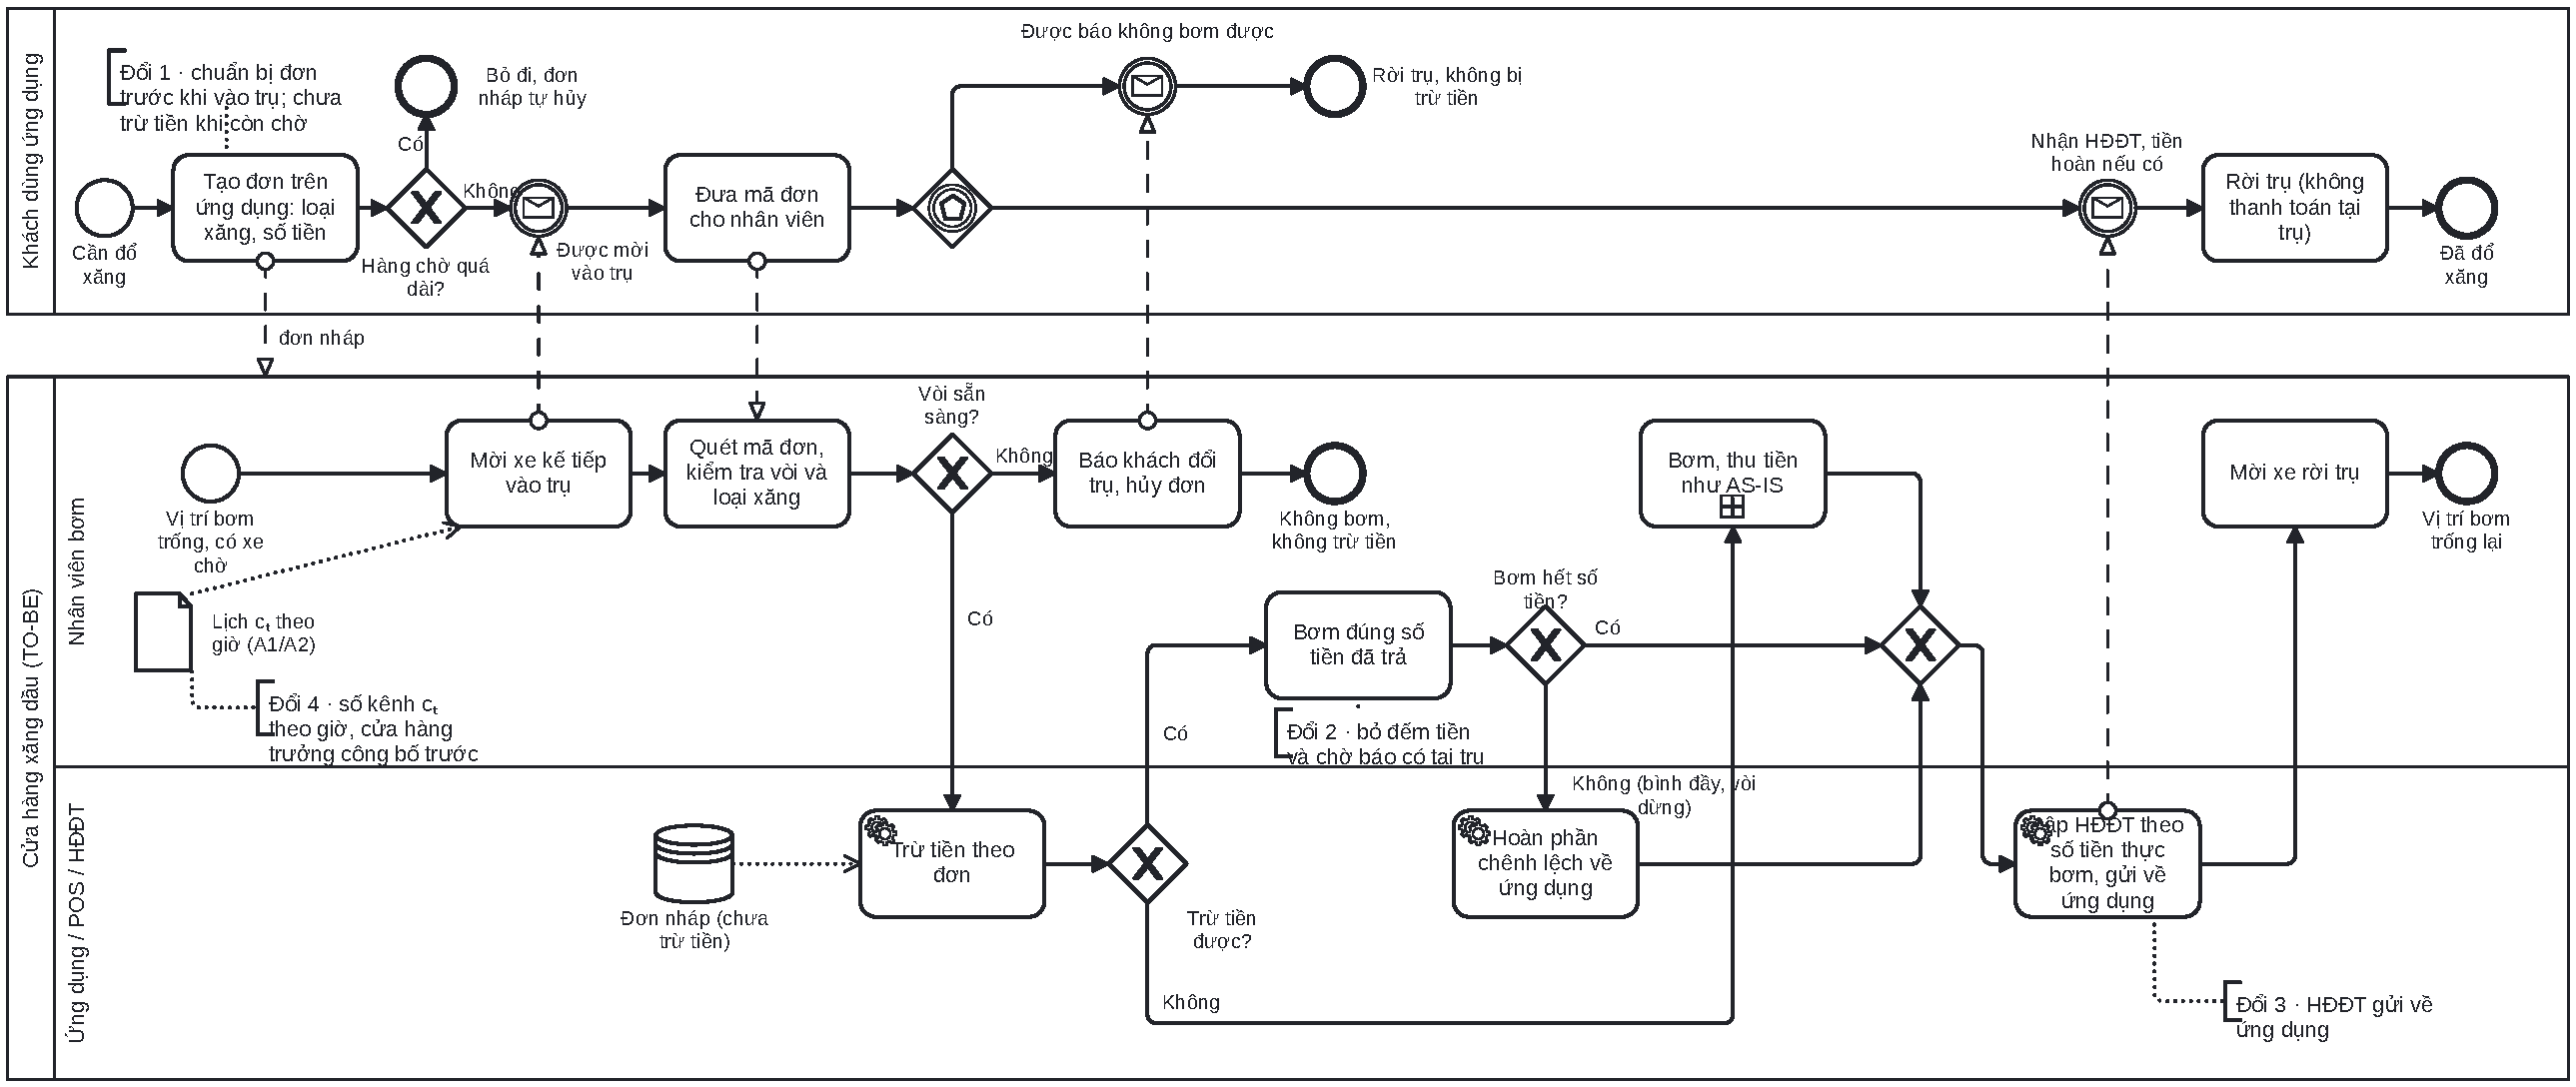
\includegraphics[width=0.86\linewidth]{figures/r1_bpmn_tobe.pdf}
\captionof{figure}{BPMN TO-BE cho khách dùng ứng dụng trả trước; ``Đổi 1--4'' là thay đổi so với AS-IS,
khối có dấu $+$ là luồng thanh toán tại trụ ở Hình~\ref{r1:bpmn}.}
\label{r1:tobe-bpmn}
{\footnotesize\textit{Nguồn: tệp \texttt{figures/r1\_bpmn\_tobe.bpmn}; Claude (Anthropic) hỗ trợ dựng
tệp BPMN, nhóm kiểm tra ký pháp theo~\cite{l3b}.}\par}
\captionof{table}{Thay đổi từ AS-IS sang TO-BE, trách nhiệm và tác động lên biến của mô hình}
\label{r1:tobe-changes}
\scriptsize
\begin{tabularx}{\linewidth}{@{}p{24mm}Y Y p{32mm}p{38mm}@{}}
\toprule
Thành phần & AS-IS & TO-BE (quy tắc vận hành) & Người chịu trách nhiệm & Tác động lên biến \\
\midrule
Số kênh theo giờ & 6 nhân viên mọi giờ & $c_t$ theo Bảng~\ref{r3:staffing}; ghép thành ca có nghỉ, báo trước; giảm kênh thì phục vụ xong xe đang bơm mới đóng vòi & Cửa hàng trưởng & $c_t$, $\rho_t$ theo giờ (A1, A2) \\
Chuẩn bị yêu cầu & Khách báo miệng tại trụ (H1) & Khách tạo đơn nháp trên ứng dụng khi còn ngoài trụ; chưa trừ tiền, bỏ đi thì đơn tự hủy & Khách; doanh nghiệp (ứng dụng) & Bớt lỗi H1, giảm $S_{\text{vào}}$ \\
Tiếp nhận tại trụ & Hỏi loại xăng, số tiền & Quét mã đơn; kiểm tra vòi \emph{trước} khi trừ tiền để không phải hoàn khi vòi lỗi & Nhân viên bơm & Tránh hoàn tiền (F2) \\
Thanh toán & Sau khi bơm: đếm tiền, trả tiền thừa hoặc chờ báo có (W2, W3) & Trừ tiền theo đơn trước khi bơm; trừ không được thì chuyển ngay sang luồng AS-IS, không giữ xe thử lại & Ứng dụng / POS; nhân viên & Giảm $S_{\text{tt}}$; $E[S]$ giảm 20\% là giả định \\
Hóa đơn và ngoại lệ & HĐĐT lập khi kết thúc bơm & HĐĐT theo số tiền thực bơm gửi về ứng dụng; bơm chưa hết số tiền thì hoàn chênh lệch tự động, đối soát cuối ngày & POS / HĐĐT; cửa hàng trưởng & Không làm tăng $S$ \\
\bottomrule
\end{tabularx}
\end{minipage}}
\end{figure}

Hai lớp thay đổi nhắm đúng hai đòn bẩy ở Mục~\ref{r1:scope}: lớp thứ nhất sửa $c_t$ (W1), lớp
thứ hai cắt $S_{\text{tt}}$ (W2, W3, F1); mức giảm 20\% của $E[S]$ tương đương thêm 1,5 kênh mỗi
giờ (Mục~\ref{r1:payment}). Thứ tự ``kiểm tra vòi rồi mới trừ tiền'' và ``đơn nháp chưa trừ tiền''
xử lý trước hai tranh chấp dễ gặp nhất của trả trước: đã trả mà không bơm được, và bỏ hàng sau khi
đặt đơn. Cần thêm một quy tắc dự phòng vì ở 08--09 và 17--19 giờ, mất một kênh đẩy $\rho_t$ lên
1,11--1,18: không bảo trì vòi trong giờ đỉnh và có nhân viên dự phòng gọi được ngay. Quy tắc này
chưa được mô phỏng, cần thử trong kế hoạch ở Bảng~\ref{r3:pilot}.

\begin{table}[htb]\centering\footnotesize
\caption{Tác động của TO-BE đến khách hàng và nhân viên: lợi ích và đánh đổi}\label{r1:tobe-impacts}
\begin{tabularx}{\linewidth}{@{}p{24mm}Y Y Y@{}}
\toprule
Bên & Lợi ích & Đánh đổi, rủi ro & Biện pháp \\
\midrule
Khách dùng ứng dụng & Ít chờ giờ đỉnh; thời gian ở trụ ngắn, không cần tiền lẻ; HĐĐT trên điện thoại & Cần điện thoại, tài khoản; tiền hoàn có độ trễ; chia sẻ dữ liệu thanh toán & Hoàn tự động, hiện trạng thái đơn; nói rõ dữ liệu được dùng làm gì \\
Khách tiền mặt & Vẫn được phục vụ; hưởng lợi gián tiếp khi hàng ngắn hơn nhờ lịch theo giờ & Thời gian ở trụ của chính họ không giảm & Giữ kênh tiền mặt, một hàng chung theo thứ tự đến \\
Nhân viên bơm & Tải đều hơn giữa các giờ; bớt đếm tiền, ít chênh lệch cuối ca & Lịch đổi theo giờ, dễ thành ca vụn; tổng giờ công giảm (96 $\to$ 88 hoặc 72 giờ/ngày); ít dư địa khi vắng người (Bảng~\ref{r3:risks}) & Ca 4--8 giờ có nghỉ, báo trước; ca dự phòng có thù lao; đào tạo quét mã, xử lý ngoại lệ \\
Cửa hàng trưởng, doanh nghiệp & Lập lịch theo dữ liệu; chi phí nhân lực thấp hơn & Thêm việc lập lịch, đối soát hoàn tiền; chi phí công nghệ (giả định 250 nghìn đồng/ngày); phụ thuộc mạng & Thử có giới hạn trước khi áp dụng rộng (Bảng~\ref{r3:pilot}) \\
\bottomrule
\end{tabularx}
\end{table}

% Nhan cu \label{r3:bpmn} khong duoc tham chieu o dau khac nen xoa duoc.
% So do: figures/r1_bpmn_tobe.bpmn (sua tren demo.bpmn.io), ban PDF: figures/r1_bpmn_tobe.pdf.

\subsection{Quy trình TO-BE và quy tắc vận hành}
\label{r1:tobe}
TO-BE gồm hai lớp thay đổi. Lớp thứ nhất áp dụng cho mọi khách: số kênh $c_t$ đổi theo
giờ theo Bảng~\ref{r3:staffing} (A1, và A2 khi có số hóa), do cửa hàng trưởng công bố
trước. Lớp thứ hai là thay đổi quy trình cho khách dùng ứng dụng (A2): đơn được chuẩn bị
trước khi vào trụ, tại trụ nhân viên chỉ quét mã, kiểm tra vòi, hệ thống trừ tiền rồi
mới bơm đúng số tiền; HĐĐT gửi về ứng dụng. Khách không dùng ứng dụng, hoặc trừ tiền
không thành công, đi theo luồng AS-IS ở Hình~\ref{r1:bpmn}, nên kênh tiền mặt vẫn được giữ.
Hình~\ref{r1:tobe-bpmn} và Bảng~\ref{r1:tobe-changes} cho biết bước nào đổi, ai chịu
trách nhiệm và thay đổi tác động lên biến nào của mô hình.

\begin{figure}[p]\centering
\rotatebox{90}{\begin{minipage}{\textheight}\centering
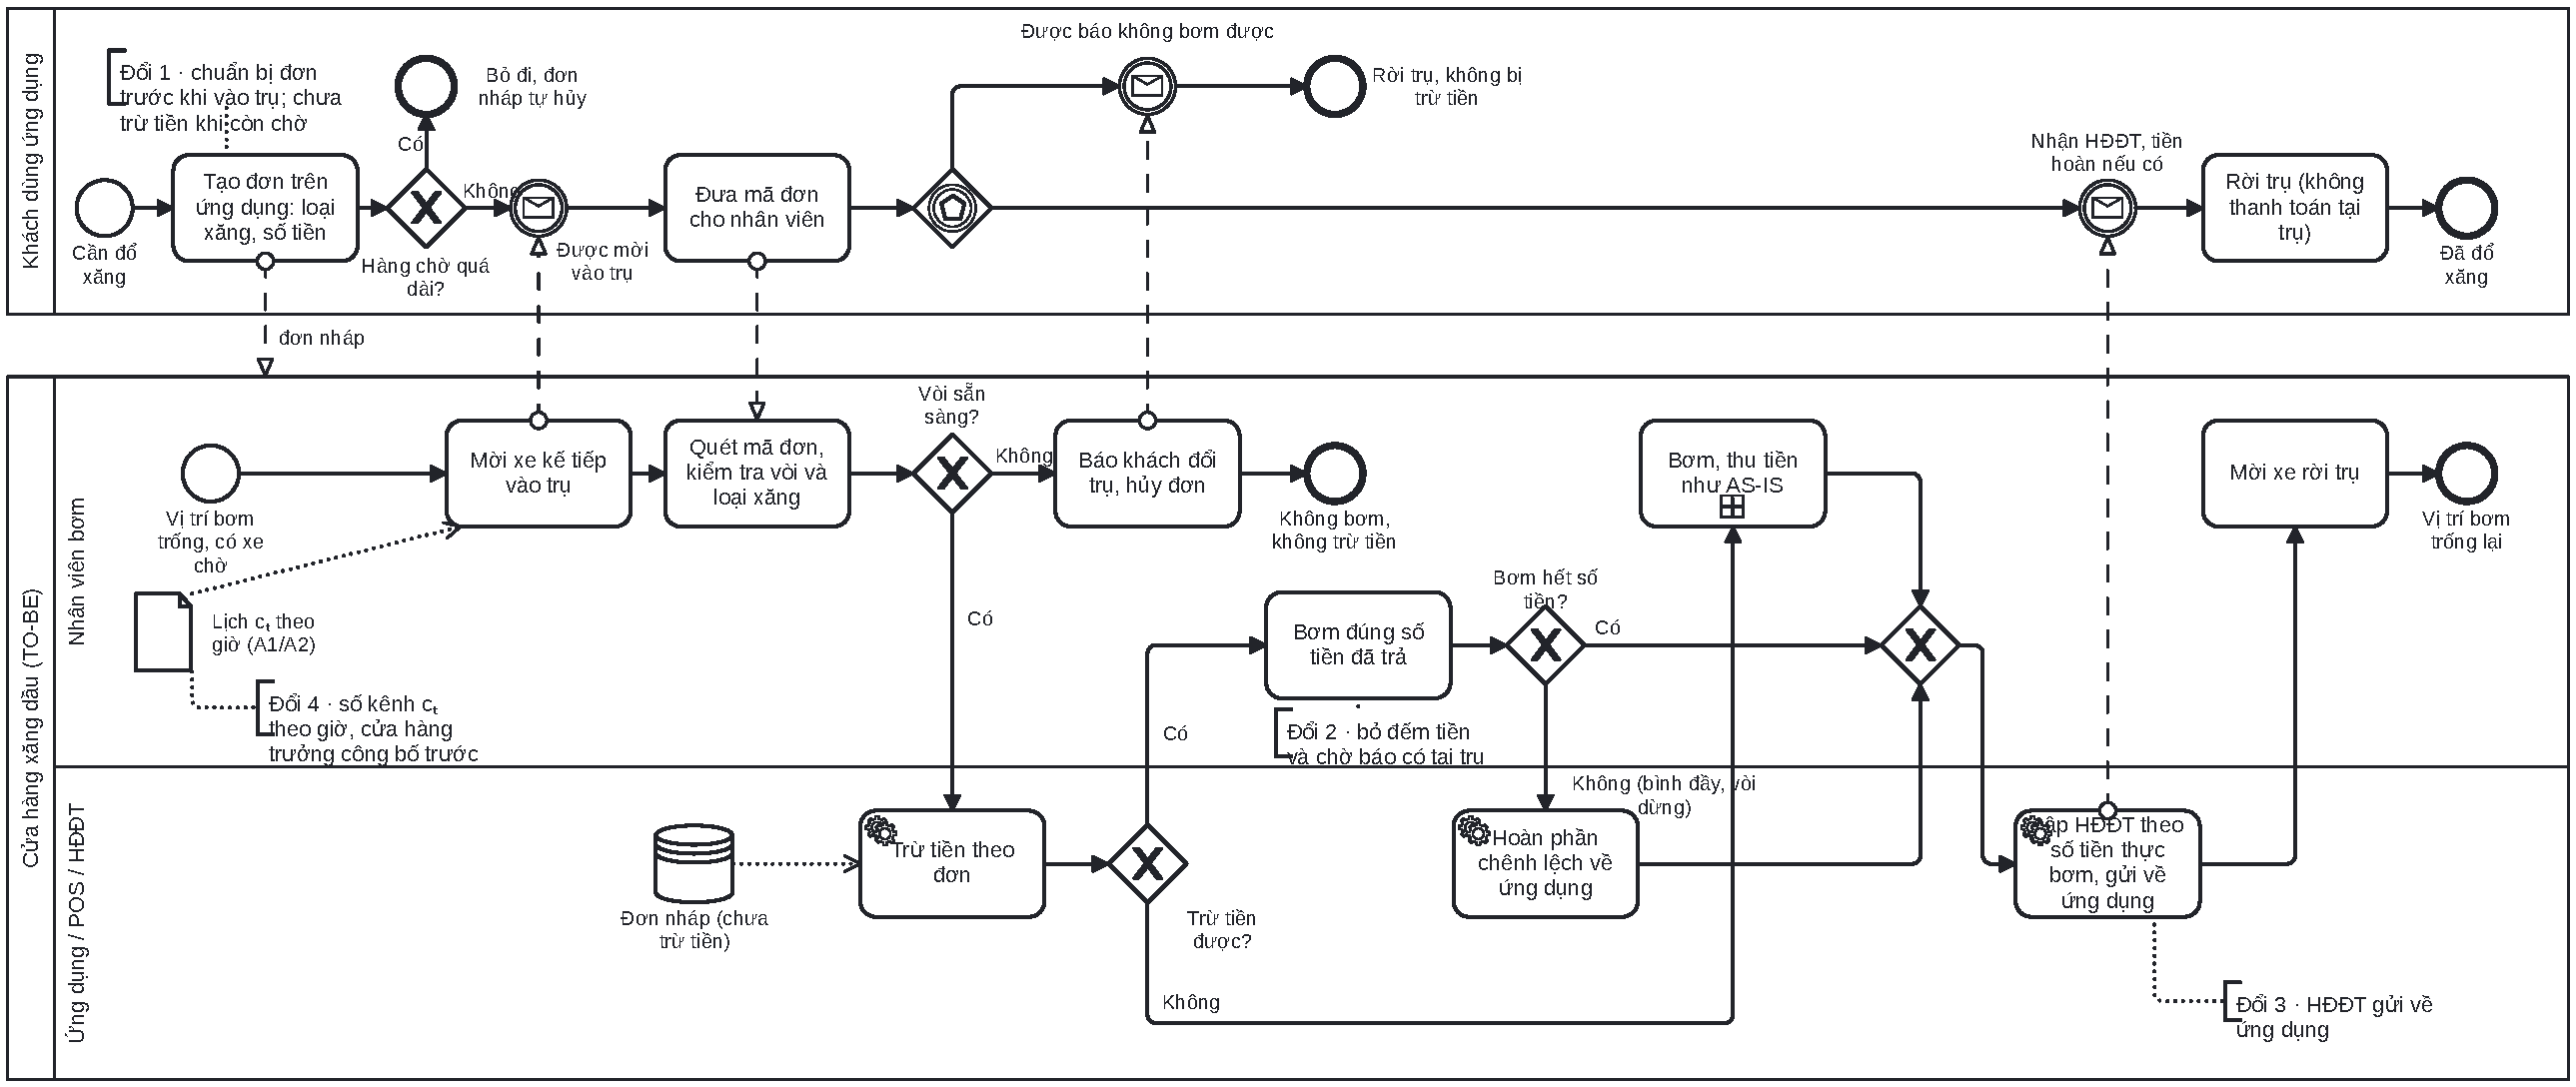
\includegraphics[width=0.86\linewidth]{figures/r1_bpmn_tobe.pdf}
\captionof{figure}{BPMN TO-BE cho khách dùng ứng dụng trả trước; ``Đổi 1--4'' là thay đổi so với AS-IS,
khối có dấu $+$ là luồng thanh toán tại trụ ở Hình~\ref{r1:bpmn}.}
\label{r1:tobe-bpmn}
{\footnotesize\textit{Nguồn: tệp \texttt{figures/r1\_bpmn\_tobe.bpmn}; Claude (Anthropic) hỗ trợ dựng
tệp BPMN, nhóm kiểm tra ký pháp theo~\cite{l3b}.}\par}
\captionof{table}{Thay đổi từ AS-IS sang TO-BE, trách nhiệm và tác động lên biến của mô hình}
\label{r1:tobe-changes}
\scriptsize
\begin{tabularx}{\linewidth}{@{}p{24mm}Y Y p{32mm}p{38mm}@{}}
\toprule
Thành phần & AS-IS & TO-BE (quy tắc vận hành) & Người chịu trách nhiệm & Tác động lên biến \\
\midrule
Số kênh theo giờ & 6 nhân viên mọi giờ & $c_t$ theo Bảng~\ref{r3:staffing}; ghép thành ca có nghỉ, báo trước; giảm kênh thì phục vụ xong xe đang bơm mới đóng vòi & Cửa hàng trưởng & $c_t$, $\rho_t$ theo giờ (A1, A2) \\
Chuẩn bị yêu cầu & Khách báo miệng tại trụ (H1) & Khách tạo đơn nháp trên ứng dụng khi còn ngoài trụ; chưa trừ tiền, bỏ đi thì đơn tự hủy & Khách; doanh nghiệp (ứng dụng) & Bớt lỗi H1, giảm $S_{\text{vào}}$ \\
Tiếp nhận tại trụ & Hỏi loại xăng, số tiền & Quét mã đơn; kiểm tra vòi \emph{trước} khi trừ tiền để không phải hoàn khi vòi lỗi & Nhân viên bơm & Tránh hoàn tiền (F2) \\
Thanh toán & Sau khi bơm: đếm tiền, trả tiền thừa hoặc chờ báo có (W2, W3) & Trừ tiền theo đơn trước khi bơm; trừ không được thì chuyển ngay sang luồng AS-IS, không giữ xe thử lại & Ứng dụng / POS; nhân viên & Giảm $S_{\text{tt}}$; $E[S]$ giảm 20\% là giả định \\
Hóa đơn và ngoại lệ & HĐĐT lập khi kết thúc bơm & HĐĐT theo số tiền thực bơm gửi về ứng dụng; bơm chưa hết số tiền thì hoàn chênh lệch tự động, đối soát cuối ngày & POS / HĐĐT; cửa hàng trưởng & Không làm tăng $S$ \\
\bottomrule
\end{tabularx}
\end{minipage}}
\end{figure}

Hai lớp thay đổi nhắm đúng hai đòn bẩy ở Mục~\ref{r1:scope}: lớp thứ nhất sửa $c_t$ (W1), lớp
thứ hai cắt $S_{\text{tt}}$ (W2, W3, F1); mức giảm 20\% của $E[S]$ tương đương thêm 1,5 kênh mỗi
giờ (Mục~\ref{r1:payment}). Thứ tự ``kiểm tra vòi rồi mới trừ tiền'' và ``đơn nháp chưa trừ tiền''
xử lý trước hai tranh chấp dễ gặp nhất của trả trước: đã trả mà không bơm được, và bỏ hàng sau khi
đặt đơn. Cần thêm một quy tắc dự phòng vì ở 08--09 và 17--19 giờ, mất một kênh đẩy $\rho_t$ lên
1,11--1,18: không bảo trì vòi trong giờ đỉnh và có nhân viên dự phòng gọi được ngay. Quy tắc này
chưa được mô phỏng, cần thử trong kế hoạch ở Bảng~\ref{r3:pilot}.

\begin{table}[htb]\centering\footnotesize
\caption{Tác động của TO-BE đến khách hàng và nhân viên: lợi ích và đánh đổi}\label{r1:tobe-impacts}
\begin{tabularx}{\linewidth}{@{}p{24mm}Y Y Y@{}}
\toprule
Bên & Lợi ích & Đánh đổi, rủi ro & Biện pháp \\
\midrule
Khách dùng ứng dụng & Ít chờ giờ đỉnh; thời gian ở trụ ngắn, không cần tiền lẻ; HĐĐT trên điện thoại & Cần điện thoại, tài khoản; tiền hoàn có độ trễ; chia sẻ dữ liệu thanh toán & Hoàn tự động, hiện trạng thái đơn; nói rõ dữ liệu được dùng làm gì \\
Khách tiền mặt & Vẫn được phục vụ; hưởng lợi gián tiếp khi hàng ngắn hơn nhờ lịch theo giờ & Thời gian ở trụ của chính họ không giảm & Giữ kênh tiền mặt, một hàng chung theo thứ tự đến \\
Nhân viên bơm & Tải đều hơn giữa các giờ; bớt đếm tiền, ít chênh lệch cuối ca & Lịch đổi theo giờ, dễ thành ca vụn; tổng giờ công giảm (96 $\to$ 88 hoặc 72 giờ/ngày); ít dư địa khi vắng người (Bảng~\ref{r3:risks}) & Ca 4--8 giờ có nghỉ, báo trước; ca dự phòng có thù lao; đào tạo quét mã, xử lý ngoại lệ \\
Cửa hàng trưởng, doanh nghiệp & Lập lịch theo dữ liệu; chi phí nhân lực thấp hơn & Thêm việc lập lịch, đối soát hoàn tiền; chi phí công nghệ (giả định 250 nghìn đồng/ngày); phụ thuộc mạng & Thử có giới hạn trước khi áp dụng rộng (Bảng~\ref{r3:pilot}) \\
\bottomrule
\end{tabularx}
\end{table}

% Nhan cu \label{r3:bpmn} khong duoc tham chieu o dau khac nen xoa duoc.
% So do: figures/r1_bpmn_tobe.bpmn (sua tren demo.bpmn.io), ban PDF: figures/r1_bpmn_tobe.pdf.

\subsection{Quy trình TO-BE và quy tắc vận hành}
\label{r1:tobe}
TO-BE gồm hai lớp thay đổi. Lớp thứ nhất áp dụng cho mọi khách: số kênh $c_t$ đổi theo
giờ theo Bảng~\ref{r3:staffing} (A1, và A2 khi có số hóa), do cửa hàng trưởng công bố
trước. Lớp thứ hai là thay đổi quy trình cho khách dùng ứng dụng (A2): đơn được chuẩn bị
trước khi vào trụ, tại trụ nhân viên chỉ quét mã, kiểm tra vòi, hệ thống trừ tiền rồi
mới bơm đúng số tiền; HĐĐT gửi về ứng dụng. Khách không dùng ứng dụng, hoặc trừ tiền
không thành công, đi theo luồng AS-IS ở Hình~\ref{r1:bpmn}, nên kênh tiền mặt vẫn được giữ.
Hình~\ref{r1:tobe-bpmn} và Bảng~\ref{r1:tobe-changes} cho biết bước nào đổi, ai chịu
trách nhiệm và thay đổi tác động lên biến nào của mô hình.

\begin{figure}[p]\centering
\rotatebox{90}{\begin{minipage}{\textheight}\centering
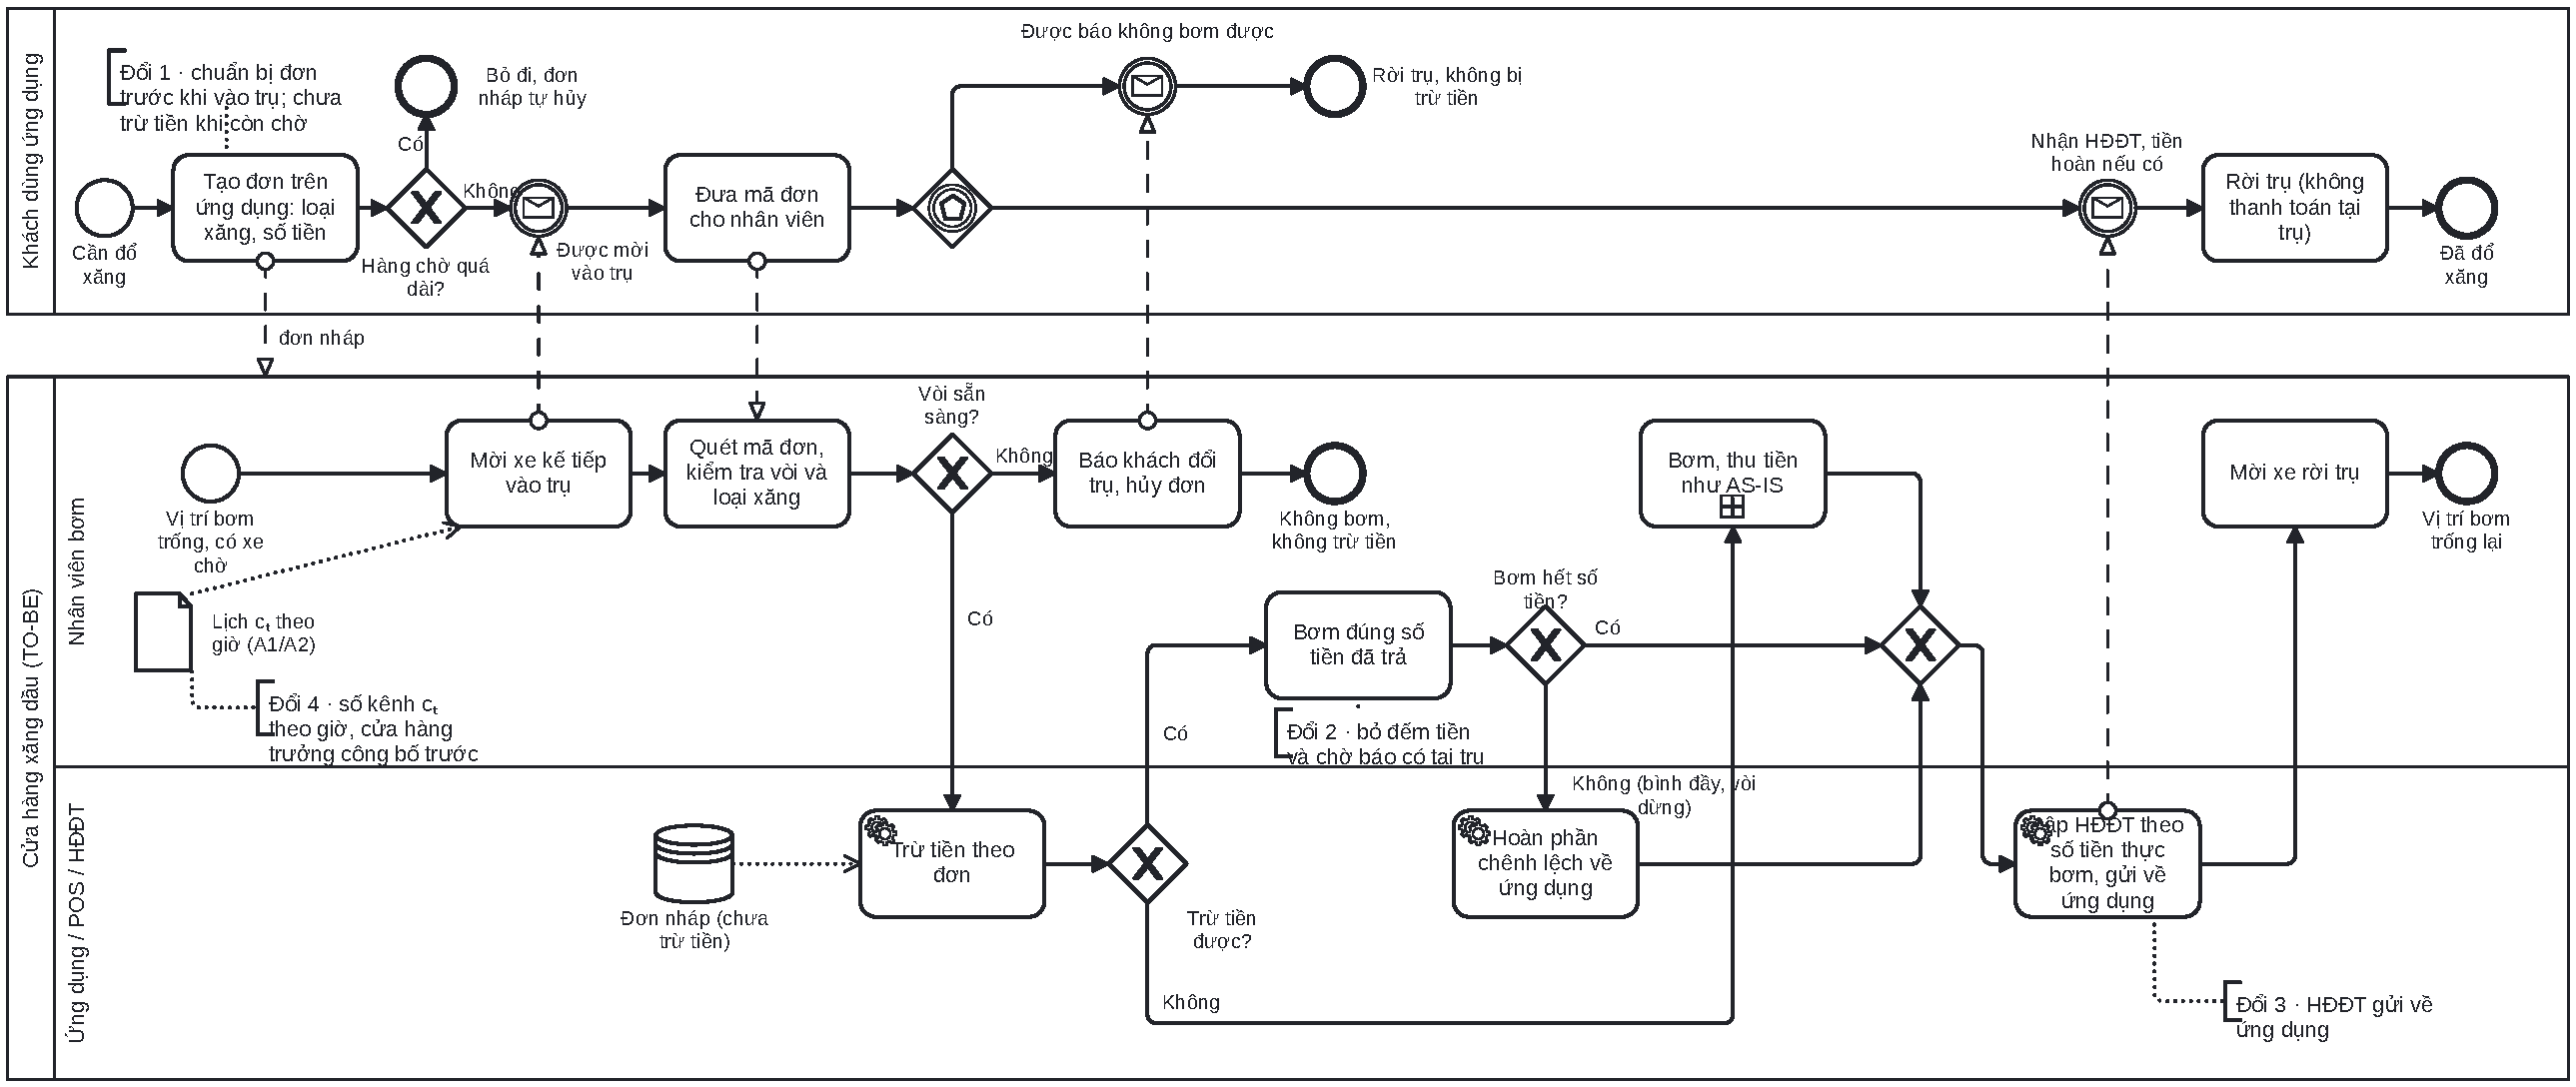
\includegraphics[width=0.86\linewidth]{figures/r1_bpmn_tobe.pdf}
\captionof{figure}{BPMN TO-BE cho khách dùng ứng dụng trả trước; ``Đổi 1--4'' là thay đổi so với AS-IS,
khối có dấu $+$ là luồng thanh toán tại trụ ở Hình~\ref{r1:bpmn}.}
\label{r1:tobe-bpmn}
{\footnotesize\textit{Nguồn: tệp \texttt{figures/r1\_bpmn\_tobe.bpmn}; Claude (Anthropic) hỗ trợ dựng
tệp BPMN, nhóm kiểm tra ký pháp theo~\cite{l3b}.}\par}
\captionof{table}{Thay đổi từ AS-IS sang TO-BE, trách nhiệm và tác động lên biến của mô hình}
\label{r1:tobe-changes}
\scriptsize
\begin{tabularx}{\linewidth}{@{}p{24mm}Y Y p{32mm}p{38mm}@{}}
\toprule
Thành phần & AS-IS & TO-BE (quy tắc vận hành) & Người chịu trách nhiệm & Tác động lên biến \\
\midrule
Số kênh theo giờ & 6 nhân viên mọi giờ & $c_t$ theo Bảng~\ref{r3:staffing}; ghép thành ca có nghỉ, báo trước; giảm kênh thì phục vụ xong xe đang bơm mới đóng vòi & Cửa hàng trưởng & $c_t$, $\rho_t$ theo giờ (A1, A2) \\
Chuẩn bị yêu cầu & Khách báo miệng tại trụ (H1) & Khách tạo đơn nháp trên ứng dụng khi còn ngoài trụ; chưa trừ tiền, bỏ đi thì đơn tự hủy & Khách; doanh nghiệp (ứng dụng) & Bớt lỗi H1, giảm $S_{\text{vào}}$ \\
Tiếp nhận tại trụ & Hỏi loại xăng, số tiền & Quét mã đơn; kiểm tra vòi \emph{trước} khi trừ tiền để không phải hoàn khi vòi lỗi & Nhân viên bơm & Tránh hoàn tiền (F2) \\
Thanh toán & Sau khi bơm: đếm tiền, trả tiền thừa hoặc chờ báo có (W2, W3) & Trừ tiền theo đơn trước khi bơm; trừ không được thì chuyển ngay sang luồng AS-IS, không giữ xe thử lại & Ứng dụng / POS; nhân viên & Giảm $S_{\text{tt}}$; $E[S]$ giảm 20\% là giả định \\
Hóa đơn và ngoại lệ & HĐĐT lập khi kết thúc bơm & HĐĐT theo số tiền thực bơm gửi về ứng dụng; bơm chưa hết số tiền thì hoàn chênh lệch tự động, đối soát cuối ngày & POS / HĐĐT; cửa hàng trưởng & Không làm tăng $S$ \\
\bottomrule
\end{tabularx}
\end{minipage}}
\end{figure}

Hai lớp thay đổi nhắm đúng hai đòn bẩy ở Mục~\ref{r1:scope}: lớp thứ nhất sửa $c_t$ (W1), lớp
thứ hai cắt $S_{\text{tt}}$ (W2, W3, F1); mức giảm 20\% của $E[S]$ tương đương thêm 1,5 kênh mỗi
giờ (Mục~\ref{r1:payment}). Thứ tự ``kiểm tra vòi rồi mới trừ tiền'' và ``đơn nháp chưa trừ tiền''
xử lý trước hai tranh chấp dễ gặp nhất của trả trước: đã trả mà không bơm được, và bỏ hàng sau khi
đặt đơn. Cần thêm một quy tắc dự phòng vì ở 08--09 và 17--19 giờ, mất một kênh đẩy $\rho_t$ lên
1,11--1,18: không bảo trì vòi trong giờ đỉnh và có nhân viên dự phòng gọi được ngay. Quy tắc này
chưa được mô phỏng, cần thử trong kế hoạch ở Bảng~\ref{r3:pilot}.

\begin{table}[htb]\centering\footnotesize
\caption{Tác động của TO-BE đến khách hàng và nhân viên: lợi ích và đánh đổi}\label{r1:tobe-impacts}
\begin{tabularx}{\linewidth}{@{}p{24mm}Y Y Y@{}}
\toprule
Bên & Lợi ích & Đánh đổi, rủi ro & Biện pháp \\
\midrule
Khách dùng ứng dụng & Ít chờ giờ đỉnh; thời gian ở trụ ngắn, không cần tiền lẻ; HĐĐT trên điện thoại & Cần điện thoại, tài khoản; tiền hoàn có độ trễ; chia sẻ dữ liệu thanh toán & Hoàn tự động, hiện trạng thái đơn; nói rõ dữ liệu được dùng làm gì \\
Khách tiền mặt & Vẫn được phục vụ; hưởng lợi gián tiếp khi hàng ngắn hơn nhờ lịch theo giờ & Thời gian ở trụ của chính họ không giảm & Giữ kênh tiền mặt, một hàng chung theo thứ tự đến \\
Nhân viên bơm & Tải đều hơn giữa các giờ; bớt đếm tiền, ít chênh lệch cuối ca & Lịch đổi theo giờ, dễ thành ca vụn; tổng giờ công giảm (96 $\to$ 88 hoặc 72 giờ/ngày); ít dư địa khi vắng người (Bảng~\ref{r3:risks}) & Ca 4--8 giờ có nghỉ, báo trước; ca dự phòng có thù lao; đào tạo quét mã, xử lý ngoại lệ \\
Cửa hàng trưởng, doanh nghiệp & Lập lịch theo dữ liệu; chi phí nhân lực thấp hơn & Thêm việc lập lịch, đối soát hoàn tiền; chi phí công nghệ (giả định 250 nghìn đồng/ngày); phụ thuộc mạng & Thử có giới hạn trước khi áp dụng rộng (Bảng~\ref{r3:pilot}) \\
\bottomrule
\end{tabularx}
\end{table}
